To quantify the stability and availability of the system I presented it with a number of scenarios in various tests. I will only report the setup and whether a test succeeded for the simpler scenarios. For the more challenging test I will present a more detailed look at system performance which will allow us to discuss their conclusions in the next section.

The most basic tests checks the file system functions and is consistent with these steps: 
\begin{enumerate}
	\item Use the \textit{mkdir} command to build a small flat directory tree of $10$ directories on the cluster.
	\item Querying the content of the cluster using the \textit{ls} command. 
	\item Check these answer matches with the mkdir orders from step one.
	\item Remove the directories using \textit{rm}.
	\item Again query the content of the cluster.
	\item Check the answer to verify the cluster is now empty.
\end{enumerate}
All the commands are send from a single client. The writeserver will redirect any request for the clusters content to a random readserver. This means if the test succeeds we know the changes are propagated to at least one readserver. The test ran without problems for $10$ runs giving a high chance the changes propagate to all readservers.

For the second test I focussed on the availability of the cluster. While the cluster was running without processing any client request the writeserver was killed using \textsc{SIGKILL} before running the first test. If the first test still completes a new master must have been elected and accepted. This test succeeded without problems.

As third test I focussed on the stability and performance of the system under trivial load. A single machine send out $300$ \textit{mkdir} requests sequentially. These tests failed every time. From the logs we can plot the time left till the writeservers heartbeat times out, see \cref{fig:hbt}.

\begin{figure}[htbp]
	\centering
	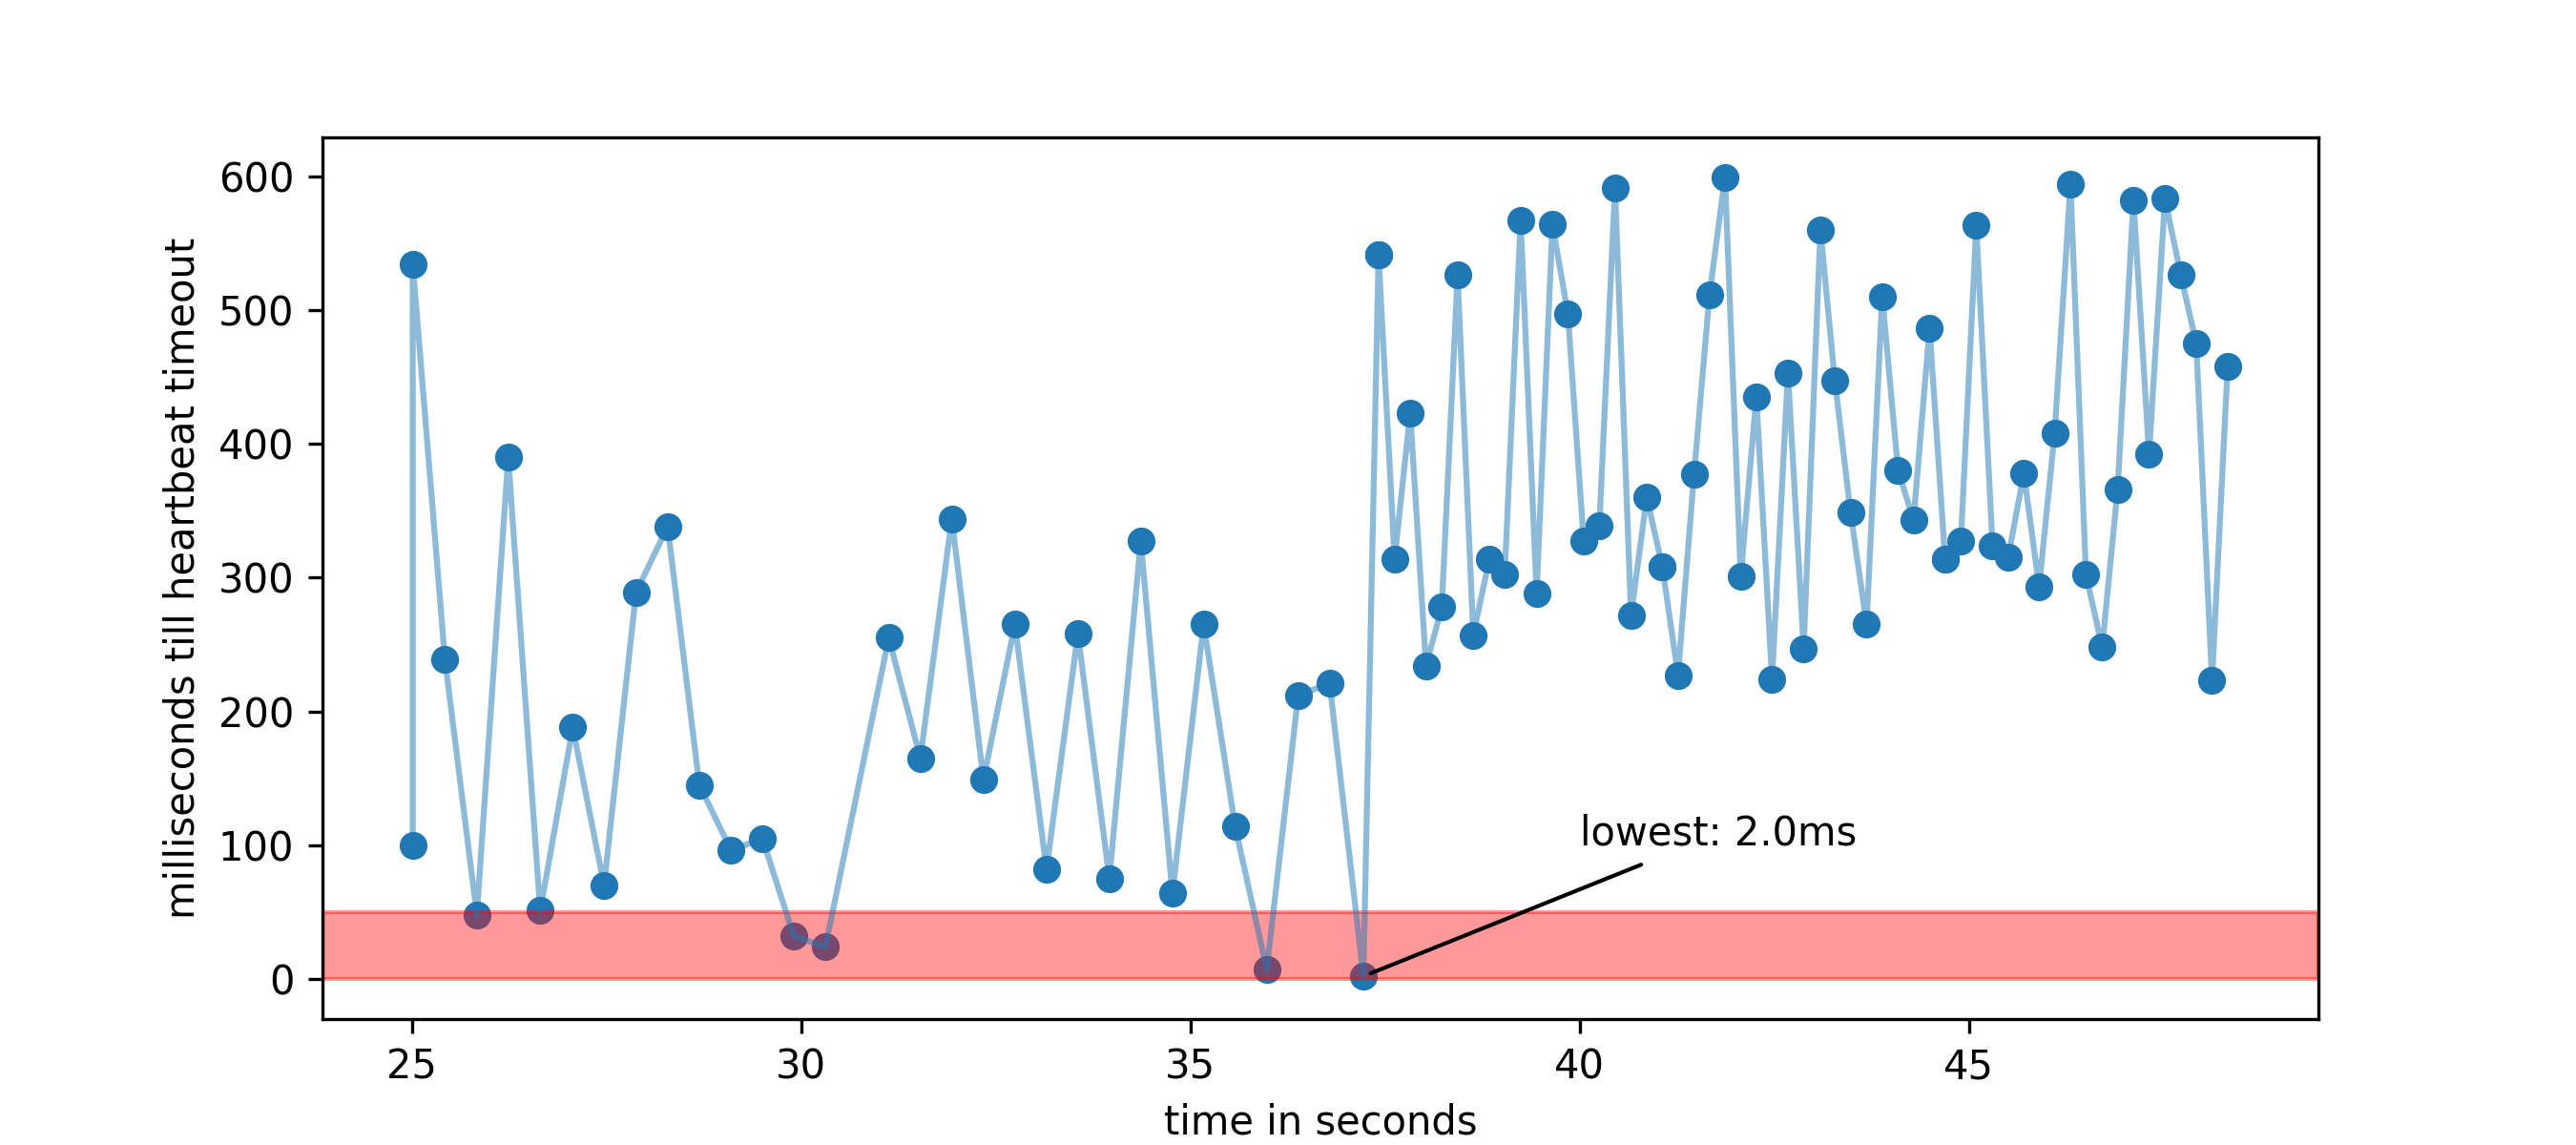
\includegraphics{../data/hb_timeout.png}
	\caption{Time left before the heartbeat times out while receiving sequential make directory requests. Around 37 seconds the writeserver timed out and a new writeserver took over because another readserver timed out. Unencumbered by the mkdir requests the new writeservers heartbeat arrive well on time.}
	\label{fig:hbt}
\end{figure}

Finally we test 'read' performance using the list directory request. I used a single client to open between 2 and 4096 simultanious connections to the cluster. Over each connection a list directory request was send 100 times. The total time between start and finish was measured for different combinations of simultaieous connections and cluster size. These times are converted to milliseconds per request. The results can be seen in \cref{fig:ls_log} and \cref{fig:ls_lin}. 
It was difficult to gather the data as larger cluster sizes often ran into heartbeat issues. Except for the run with 6 nodes the data presented here is selected from successful tests. To get this data the tests had to be run many times.
Note in \cref{fig:ls_log} as the number of requests increases the average request time goes down logarithmically. In \cref{fig:ls_lin} we see that (excluding the malfunctioning 6 node run) larger cluster sizes give shorter response times.

\begin{figure}[htbp]
	\centering
	\includegraphics{../data/ls_log.png}
	\caption{Average duration of a list directory request vs number of simultaneous connections for various cluster sizes (\#nodes). The run with 6 nodes experienced problems during its run slowing it down.}
	\label{fig:ls_log}
\end{figure}

\begin{figure}[htbp]
	\centering
	\includegraphics{../data/ls_lin.png}
	\caption{Average duration of a list directory request vs number of simultaneous connections for various cluster sizes (\#nodes). The run with 6 nodes experienced problems during its run slowing it down.}
	\label{fig:ls_lin}
\end{figure}
